\documentclass[11pt, a4paper]{article}
\usepackage{subfiles}

% Algorithms
	%\usepackage{algpseudocode}
	%\usepackage{algorithm}

% Babel
\usepackage[english]{babel}

% Code writing
	%\usepackage[procnames]{listings}

% Font
\usepackage[utf8]{inputenc}
\usepackage[T1]{fontenc}
\usepackage{amssymb,amsmath,amsthm,amsfonts}
\usepackage{eucal}
\usepackage{textcomp}

% Footnote


% Hyperref
\usepackage[hyphens]{url}
\usepackage{cite}
\usepackage{hyperref}
\usepackage{nameref}
\usepackage{url}
% Images
\usepackage[pdftex]{graphicx}
	%\usepackage{subfigure}
\usepackage{subfig}
\usepackage{eso-pic}
\usepackage{caption}
\usepackage{wrapfig}
\usepackage{float}

% List
\usepackage{enumerate}

% SI units
\usepackage{siunitx}

% Standalone
\usepackage[subpreambles=true]{standalone}
\usepackage{import}

% Tables
\usepackage{tabularx}
\usepackage{booktabs}
\usepackage{multirow}

% TiKz and graphs
\usepackage{pgf,tikz,pgfplots}
% \usepackage{gnuplottex}
\usepackage{bm}
\usepackage{relsize}
%\usepackage[compat=1.1.0]{tikz-feynman}
\usepackage{circuitikz}

% Typeset
%\usepackage[top=2cm,bottom=2cm,left=2cm,right=2cm]{geometry}
\usepackage[top=2cm,bottom=2cm,left=2cm,right=2cm]{geometry}
\usepackage{fancyhdr}
\usepackage{indentfirst}
\usepackage{titlesec}
\usepackage{setspace}
\usepackage{xspace}
% \usepackage{parskip}  % Elimina il separatore a inizio paragrafo
\usepackage{afterpage}
\usepackage{comment}

%Python
\usepackage{xcolor}
\usepackage{listings}
\usepackage{framed}

%Per scrivere matrice identità
\usepackage{bbold}
%Per semplificazione formule
\usepackage{cancel}

%Evidenziare formule
\usepackage{empheq}
	%oppure
	%\usepackage{xcolor}
\usepackage{soul}

%Evidenziare testo con mdframed
\usepackage{mdframed}

%Note a margine
\usepackage{marginnote}

%Display data
\usepackage{datetime}

%Physics
\usepackage{physics}
%Geometry
%\newgeometry{inner=20mm,
%            outer=49mm,% = marginparsep + marginparwidth
%                       %   + 5mm (between marginpar and page border)
%            top=20mm,
%            bottom=25mm,
%            marginparsep=6mm,
%            marginparwidth=30mm}
%\makeatletter
%\renewcommand{\@marginparreset}{%
%  \reset@font\small
%  \raggedright
%  \slshape
%  \@setminipage
%}
%\makeatother

%Atom Latex
%\pgfplotsset{compat=1.15}

%%
\captionsetup[table]{font=small,labelfont={bf},skip=10pt}
\captionsetup[figure]{font=small,labelfont={bf},skip=10pt}

%intestazione pagina
%\pagestyle{fancy}
%\fancyhf{}
%\fancyhead[RE]{\ifnum\value{chapter}>0\nouppercase{\leftmark}\fi}
%\fancyhead[LE]{\small\textbf{\thepage}}
%\fancyhead[LO]{\nouppercase{\rightmark}}
%\fancyhead[RO]{\small\textbf{\thepage}}

%link ipertestuale per indice
\hypersetup{
	colorlinks=false,
	linkcolor=black,
	filecolor=blue,
	citecolor = blue,
	urlcolor=blue,
	}

%%%%%indent%%%
\setlength{\parindent}{15pt}
\setlength{\parskip}{0pt}


%boh
%\renewcommand{\chaptermark}[1]{%
% \markboth{\MakeUppercase{%
% \chaptername}\ \thechapter.%
% \ #1}{}}


 %Python in latex
 \definecolor{codegreen}{rgb}{0,0.6,0}
\definecolor{codegray}{rgb}{0.5,0.5,0.5}
\definecolor{codepurple}{rgb}{0.58,0,0.82}
\definecolor{backcolour}{rgb}{0.95,0.95,0.92}
\definecolor{commentcolour}{rgb}{0.43,0.63,0.65}

\definecolor{shadecolor}{rgb}{0.93, 0.93, 0.93}
\definecolor{darkgreen}{rgb}{0.0, 0.5, 0.0}
\definecolor{darkred}{rgb}{0.8, 0.0, 0.0}
\definecolor{violet}{rgb}{0.55, 0.0, 0.55}

\lstdefinestyle{mystyle}{ %Stile python code
    backgroundcolor=\color{shadecolor},
    commentstyle=\color{commentcolour},
    keywordstyle=\color{darkgreen},
    numberstyle=\tiny\color{codegray},
    stringstyle=\color{darkred},
    basicstyle=\footnotesize\ttfamily,
    breakatwhitespace=false,
    breaklines=true,
    captionpos=b,
    keepspaces=true,
    numbers=left,
    numbersep=5pt,
    showspaces=false,
    showstringspaces=false,
    showtabs=false,
    tabsize=4
}

\definecolor{vgreen}{RGB}{104,180,104}
\definecolor{vblue}{RGB}{49,49,255}
\definecolor{vorange}{RGB}{255,143,102}

%verilog in latex
\lstdefinestyle{verilog-style}
{
    language=Verilog,
    basicstyle=\small\ttfamily,
    keywordstyle=\color{vblue},
    identifierstyle=\color{black},
    commentstyle=\color{vgreen},
    numbers=left,
    numberstyle=\tiny\color{black},
    numbersep=5pt,
    tabsize=4,
    %moredelim=*[s][\colorIndex]{[}{]},
    %literate=*{:}{:}1
}

%VHDL in latex
\lstdefinestyle{VHDL-style}
{
    language=VHDL,
    basicstyle=\small\ttfamily,
    keywordstyle=\color{vblue},
    identifierstyle=\color{black},
    commentstyle=\color{vgreen},
    numbers=left,
    numberstyle=\tiny\color{black},
    numbersep=5pt,
    tabsize=4,
    %moredelim=*[s][\colorIndex]{[}{]},
    %literate=*{:}{:}1
}

\lstset{
    style=mystyle
}

%VHDL in latex
\usepackage{beramono}
\lstdefinelanguage{VHDL}{
   morekeywords={
     library,use,all,entity,is,port,in,out,end,architecture,of,
     begin,and
   },
   morecomment=[l]--
}
\colorlet{keyword}{blue!100!black!80}
\colorlet{comment}{green!90!black!90}
\lstdefinestyle{vhdl}{
   language     = VHDL,
   basicstyle   = \ttfamily\footnotesize,
   keywordstyle = \color{keyword}\bfseries,
   commentstyle = \color{comment}
}

% Derivatives
\renewcommand{\d}[0]{\mathrm{d}}
\newcommand{\dev}[2]{\displaystyle \frac{\d #1}{\d #2}}
\newcommand{\pdev}[2]{\displaystyle \frac{\partial #1}{\partial #2}}
\newcommand{\ndev}[3]{\displaystyle \frac{\d^{#3} #1}{\d #2^{#3} } }
\newcommand{\npdev}[3]{\displaystyle \frac{\partial^{#3} #1}{\partial #2^{#3} } }


%% Norms
\newcommand{\absvec}[1]{| \vec{#1} |}
\newcommand{\normvec}[1]{|\!| \vec{#1} |\!|}

\newcommand{\vmed}[1]{\left \langle #1 \right \rangle}
\newcommand{\vmedvec}[1]{\langle #1 \rangle}
\newcommand{\R}[0]{\mathbb{R}}
\renewcommand{\H}[0]{\operatorname{H}}

%Evidenziare formule
\newcommand{\mathcolorbox}[2]{\colorbox{#1}{$\displaystyle #2$}}
\newcommand{\hlfancy}[2]{\sethlcolor{#1}\hl{#2}}

%Theorem
\newtheorem{theorem}{Theorem}[section]
\newtheorem{corollary}{Corollary}[theorem]
\newtheorem{lemma}[theorem]{Lemma}
\newtheorem{proposition}[theorem]{Proposition}

\theoremstyle{definition}
\newtheorem{definition}{Definition}%[section]


%%%%%%%%%%%%%%%%%%%%Exercise and example%%%%%%%%%%%%%%%%%
\usepackage[many,most,theorems]{tcolorbox}


\newtcbtheorem{exercise}{Exercise}{ % frame stuff
    boxrule = 1pt,
    breakable,
    enhanced,
    frame empty,
    interior style= {blue!6},
    %interior empty,
    colframe=black,
    borderline ={1pt}{0pt}{black},
    left=0.2cm,
    % title stuff
    attach boxed title to top left={yshift=-2mm,xshift=0mm},
    coltitle=black,
    fonttitle=\bfseries,
    colbacktitle=white,
    boxed title style={boxrule=1pt,sharp corners}}{exercise} 

\newtcbtheorem{example}{Example}{ % frame stuff
    boxrule = 1pt,
    enhanced,
    frame empty,
    interior style= {green!6},%{left color=yellow!70,right color=green!70},
    %interior empty,
    colframe=black,
    borderline ={1pt}{0pt}{black},
    breakable,
    left=0.2cm,
    % title stuff
    attach boxed title to top left={yshift=-2mm,xshift=0mm},
    coltitle=black,
    fonttitle=\bfseries,
    colbacktitle=white,
    boxed title style={boxrule=1pt,sharp corners}}{example}
  
%\newtheorem{exercise}{Exercise}
%\newtheorem{example}{Example}

%%%%%%%%%%%%%%%%%%%%%%%%%%%%%%%%%%%

\theoremstyle{remark}
\newtheorem*{remark}{Remark}
\newtheorem{observation}{Observation}
%Evidenziare testo
\newtheorem*{solution}{Solution}

\newcommand\mybox[1]{%
  \fbox{\begin{minipage}{0.9\textwidth}#1\end{minipage}}}

  %Spiegazioni/verifiche
\newenvironment{greenbox}{\begin{mdframed}[hidealllines=true,backgroundcolor=green!20,innerleftmargin=3pt,innerrightmargin=3pt,innertopmargin=3pt,innerbottommargin=3pt]}{\end{mdframed}}

\newenvironment{bluebox}{\begin{mdframed}[hidealllines=true,backgroundcolor=blue!10,innerleftmargin=3pt,innerrightmargin=3pt,innertopmargin=3pt,innerbottommargin=3pt]}{\end{mdframed}}

\newenvironment{yellowbox}{\begin{mdframed}[hidealllines=true,backgroundcolor=yellow!20,innerleftmargin=3pt,innerrightmargin=3pt,innertopmargin=3pt,innerbottommargin=3pt]}{\end{mdframed}}

\newenvironment{redbox}{\begin{mdframed}[hidealllines=true,backgroundcolor=red!20,innerleftmargin=3pt,innerrightmargin=3pt,innertopmargin=3pt,innerbottommargin=3pt]}{\end{mdframed}}

\newenvironment{orangebox}{\begin{mdframed}[hidealllines=true,backgroundcolor=orange!20,innerleftmargin=3pt,innerrightmargin=3pt,innertopmargin=3pt,innerbottommargin=3pt]}{\end{mdframed}}

%emph equation
\newcommand*\myyellowbox[1]{%
  \colorbox{yellow!40}{\hspace{1em}#1\hspace{1em}}}

\newcommand*\mygreenbox[1]{%
  \colorbox{green!20}{\hspace{1em}#1\hspace{1em}}}


\begin{document}

\author{Sebastiano Monti\\2052399  \and Gabriele Brotolato\\2019062 \and Mario Rossi\\123456 \and Mario Rossi\\123456}
\title{\textbf{Management and Analysis of Physics Dataset (mod. A): \\ Hardware accelerated FIR filter and application to an audio stream}}
\maketitle

\section{Aim}
In this project we show an implementation of a FIR filter on an ARTY A7 FPGA, using two different architectures. For this purpose, a Digilent stereo audio Pmod I2S2 module has been used, together with I$^2$S protocol for communication with the FPGA board and an ADC/DAC ICs. 

Produced modules have been tested using Python simulations, where we generated a wave form input, together with the expected output. In addition, hardware validation has been provided using real world audio samples, analyzed through an oscilloscope.





\section{Implementation}
The used modules are listed below and the block diagram shows the various connections.
\begin{itemize}
    \item I$^2$S/AXIS interface;
    \item AXIS FIFO;
    \item FIR filter;
    \item AXIS volume controller;
    
\end{itemize}

Fig.\ref{fig:Block_diagram}.

\vspace{1cm}
\begin{figure}[h!]
    \centering
    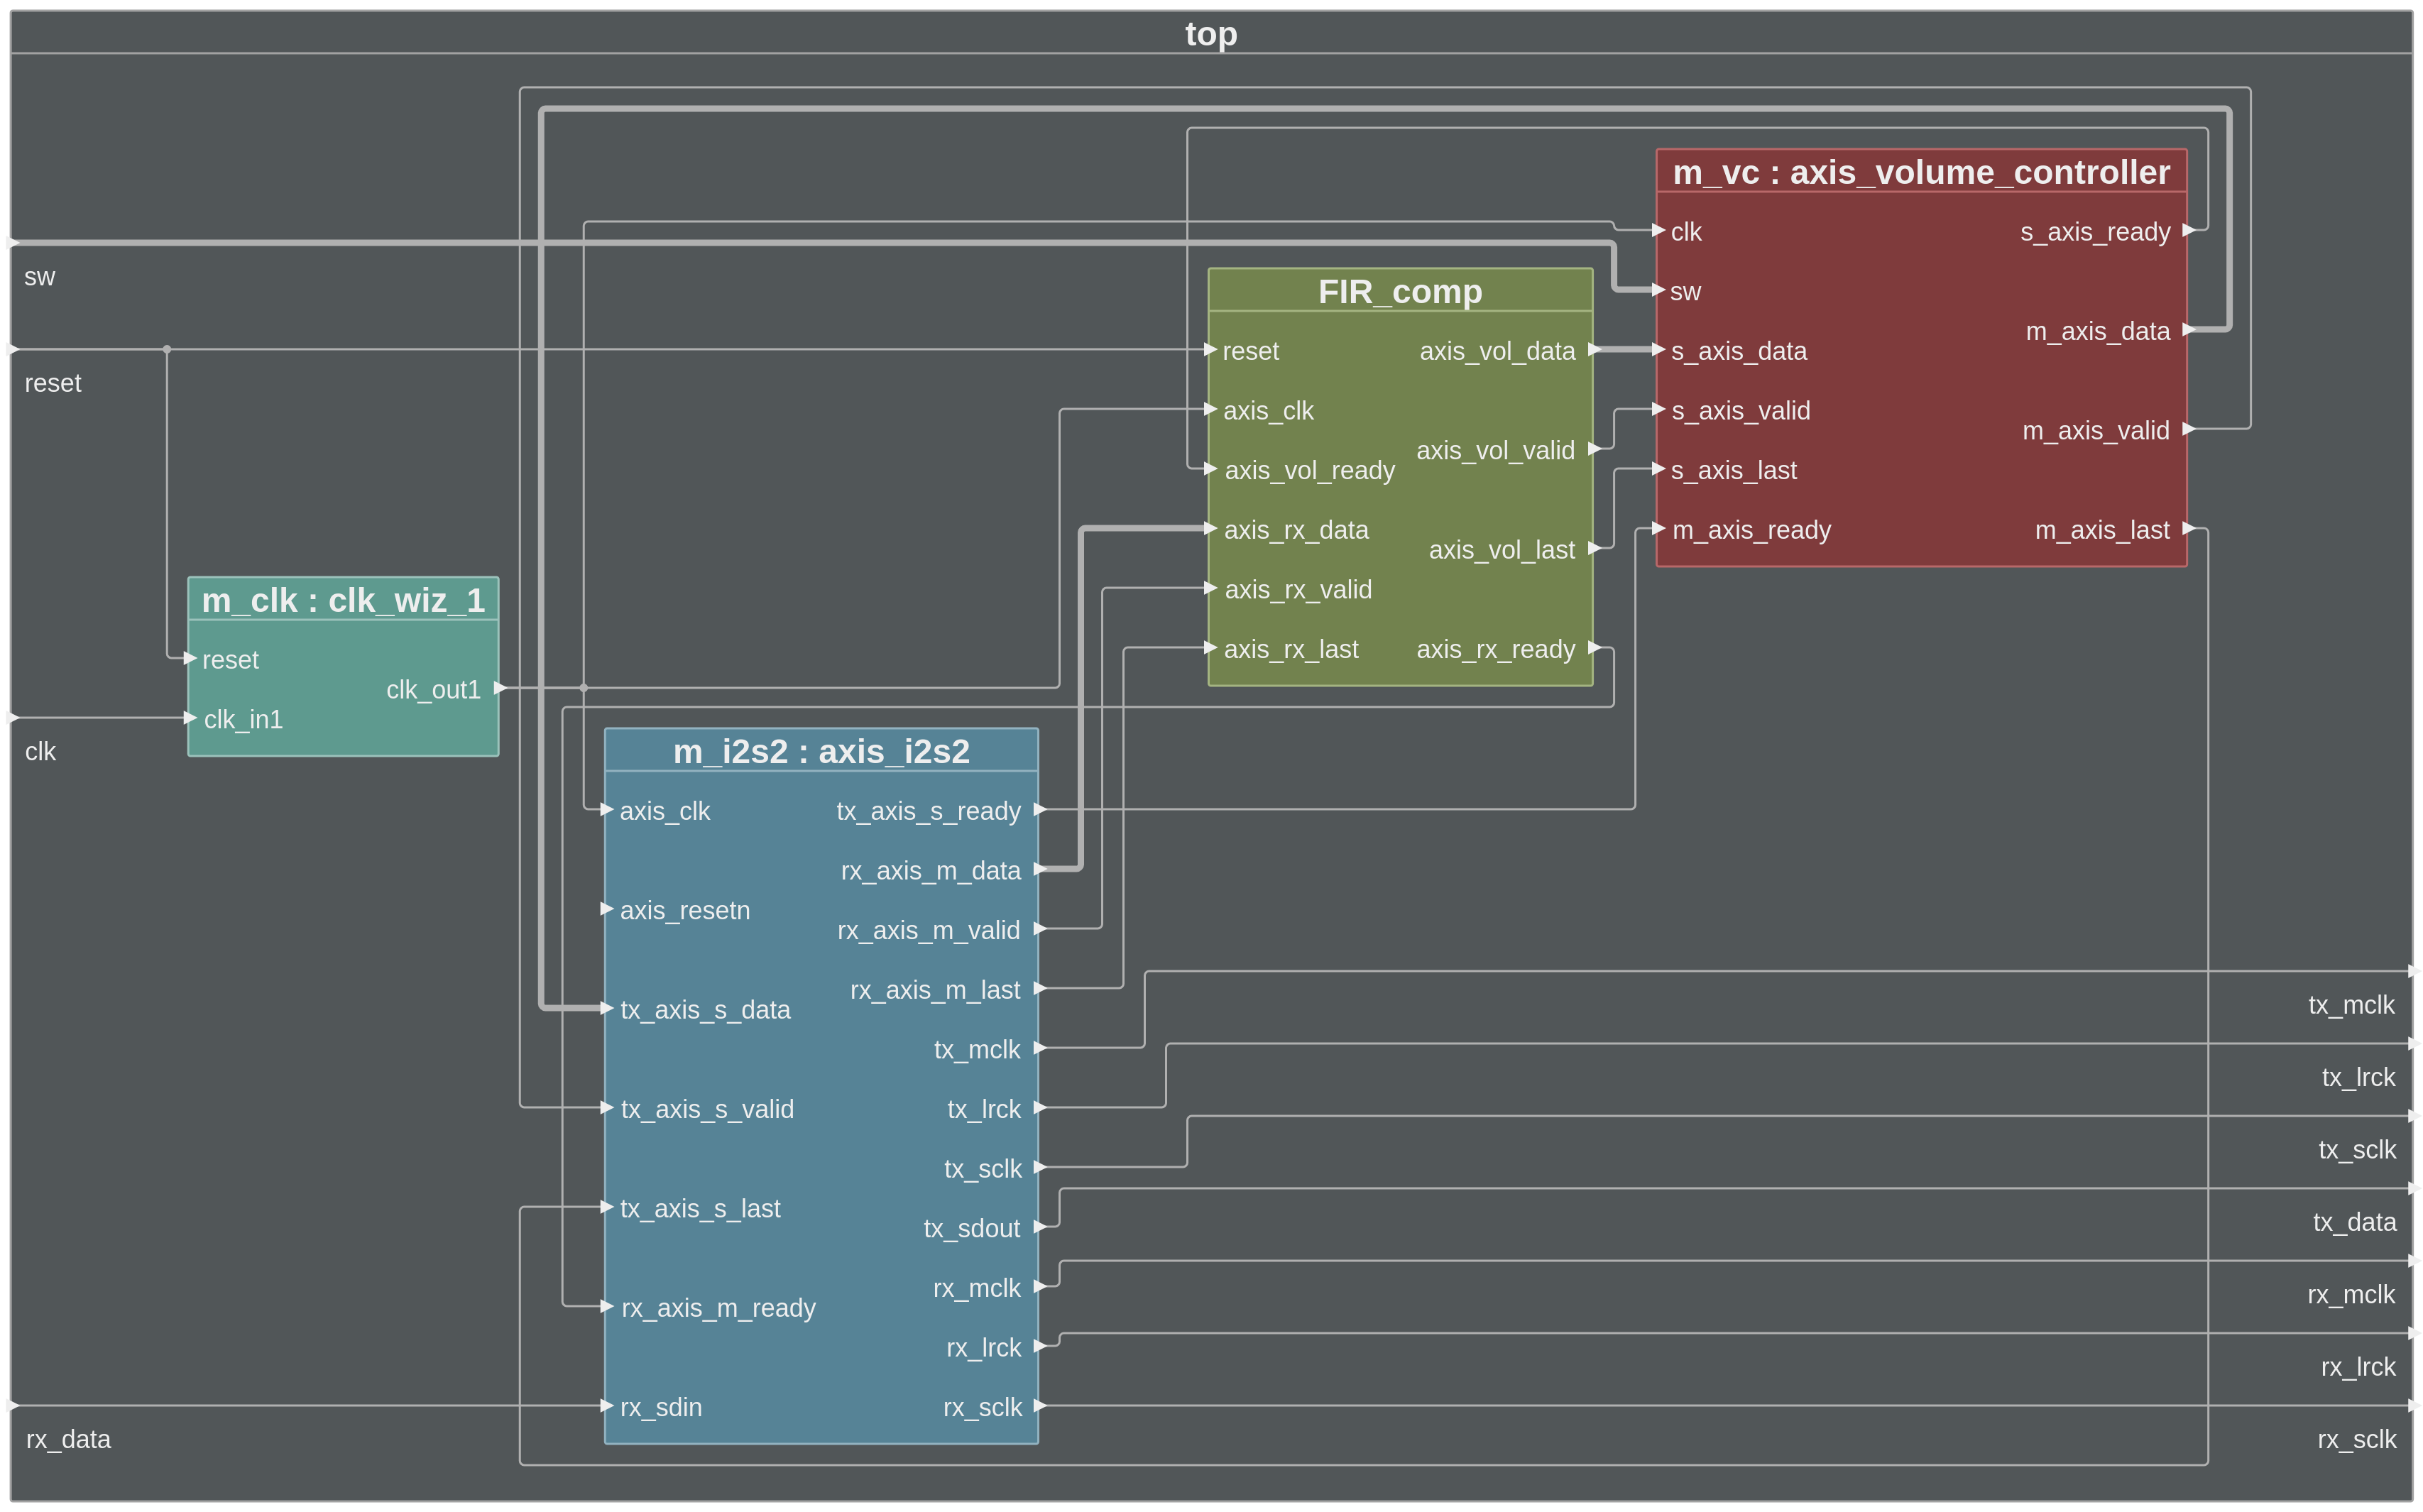
\includegraphics[width=0.8\textwidth]{images/BD_gr_cfg.png}
    \caption{\label{fig:Block_diagram} Diagram of top VHDL file.}
\end{figure}
\vspace{1cm}

In the next sections, we describe in details the structure of the main components.

\subsection{I$^2$S to AXIS interface}
The Digilent Pmod I2S2 features an audio A/D converter and a stereo D/A converter, each connected to one of two audio jacks. These circuits allow the FPGA to transmit and receive stereo audio signals via the I$^2$S protocol. In particular, input signals are translated to an AXI-Stream (encoded into the I$^2$S protocol) with the last flag used as a selector between left and right channel. The Pmod I2S2 supports 24 bit resolution per channel at input sample rates up to 108 kHz and output sample rates up to 200 kHz.

More on this module can be found on the Digilent website \cite{Digilent}. 

\subsection{FIR filter}
We implement a finite impulse response (FIR) filter, which is a filter whose impulse response is of finite duration. This module is AXI-Stream compliant and input and output FIFO are added.
%%%
We firstly provide a brief mathematical introduction. Given a sequence $\{x_i\}_{i=1,\dots,N}$ of $N$ input data samples, the output sequence of the filter is obtained by applying the following operation:
\begin{equation}
    \begin{aligned}
        y[n] &=b_{0} x[n]+b_{1} x[n-1]+\cdots+b_{k-1} x[n-k+1] \\
        &=\sum_{i=0}^{k-1} b_{i} \cdot x[n-i]
    \end{aligned}
    \label{eq:FIR}
\end{equation}
which is a convolution operation, or more simply, a weighted moving average. The $b_i$ in Eq. \ref{eq:FIR} are the coefficients that characterize the filter and its order. So, a $k$-th order filter is a filter that works with $k$ coefficients.  

%For our aims
In our work, we consider a 7-th order FIR filter. The values of the coefficients are computed through an online calculator %put ref here
, by setting a cutoff frequency of $4.8$ $kHz$ and a sample rate of $48$ $kHz$. The frequency analysis for this filter setup is showed in Figure \ref{fig:FIR_freq_analysis}.


The values of the coefficients are (16 bits signed integer format):
\begin{align*}
    b_0 &= 1915  \\
    b_1 &= 5389  \\
    b_2 &= 8266  \\
    b_3 &= 9979  \\
    b_4 &= 8266  \\
    b_5 &= 5389  \\
    b_6 &= 1915
\end{align*}

\subsubsection{Latency architecture}
This implementation is mainly focused to reduce the latency of the filter. To do so, a pipelined data flow has been employed.
%%%
First of all, we implemented a shift register that stores the last seven inputs of the data stream, using a cascade of D flip-flops.

\begin{lstlisting}[style={VHDL-style}]
shift_reg_p : process (clk) is
    begin
        if rising_edge(clk) then
            if (s_new_word = '1') then
                if (s_select = 1) then  -- right audio data 
                    audio_data_shift_r(0) <= signed(s_axis_tdata(AUDIO_DATA_WIDTH-1 downto 0));
                    audio_data_shift_r(1) <= audio_data_shift_r(0);
                    audio_data_shift_r(2) <= audio_data_shift_r(1);
                    audio_data_shift_r(3) <= audio_data_shift_r(2);
                    audio_data_shift_r(4) <= audio_data_shift_r(3);
                    audio_data_shift_r(5) <= audio_data_shift_r(4);
                    audio_data_shift_r(6) <= audio_data_shift_r(5);
                else    -- left audio data
                    audio_data_shift_l(0) <= signed(s_axis_tdata(AUDIO_DATA_WIDTH-1 downto 0));
                    audio_data_shift_l(1) <= audio_data_shift_l(0);
                    audio_data_shift_l(2) <= audio_data_shift_l(1);
                    audio_data_shift_l(3) <= audio_data_shift_l(2);
                    audio_data_shift_l(4) <= audio_data_shift_l(3);
                    audio_data_shift_l(5) <= audio_data_shift_l(4);
                    audio_data_shift_l(6) <= audio_data_shift_l(5);
                end if;
            end if;
        end if;

    end process shift_reg_p;
\end{lstlisting}

When the data are stored, the multiplication can take place. Here the whole 7 samples are processed, and finally, on the following clock cycle, the addition is performed.

\begin{lstlisting}[style={VHDL-style}]
process (clk) is
begin
   if rising_edge(clk) then
       if (s_new_packet_r(0) = '1') then  -- multiplication
            
           mult_reg_l(0) <= audio_data_shift_l(0) * to_signed(coeff(0), 16);
           mult_reg_l(1) <= audio_data_shift_l(1) * to_signed(coeff(1), 16);
           mult_reg_l(2) <= audio_data_shift_l(2) * to_signed(coeff(2), 16);
           mult_reg_l(3) <= audio_data_shift_l(3) * to_signed(coeff(3), 16);
           mult_reg_l(4) <= audio_data_shift_l(4) * to_signed(coeff(4), 16);
           mult_reg_l(5) <= audio_data_shift_l(5) * to_signed(coeff(5), 16);
           mult_reg_l(6) <= audio_data_shift_l(6) * to_signed(coeff(6), 16);

           mult_reg_r(0) <= audio_data_shift_r(0) * to_signed(coeff(0), 16);
           mult_reg_r(1) <= audio_data_shift_r(1) * to_signed(coeff(1), 16);
           mult_reg_r(2) <= audio_data_shift_r(2) * to_signed(coeff(2), 16);
           mult_reg_r(3) <= audio_data_shift_r(3) * to_signed(coeff(3), 16);
           mult_reg_r(4) <= audio_data_shift_r(4) * to_signed(coeff(4), 16);
           mult_reg_r(5) <= audio_data_shift_r(5) * to_signed(coeff(5), 16);
           mult_reg_r(6) <= audio_data_shift_r(6) * to_signed(coeff(6), 16);

        elsif (s_new_packet_r(1) = '1') then  -- addition
            data(0) <= mult_reg_l(0) + mult_reg_l(1) + mult_reg_l(2)
 + mult_reg_l(3) + mult_reg_l(4) + mult_reg_l(5) + mult_reg_l(6);
            data(1) <= mult_reg_r(0) + mult_reg_r(1) + mult_reg_r(2)
 + mult_reg_r(3) + mult_reg_r(4) + mult_reg_r(5) + mult_reg_r(6);
        end if;
    end if;
end process;
\end{lstlisting}

From the code above it is clear that in two clock cycles the data are processed, but the price in resources is very high. In this particular case, 14 DSP blocks are used (the ARTY A/ 35T has got 90 DSPs).

%% table with resources utilization

\subsubsection{Multiplication and Accumulation (MAC) architecture}

In this second architecture, the principle remains the same, but the accumulation is split in seven different steps. In our case, we used a FSM that multiplies and accumulates all the seven steps.  
In this way, only 2 DSPs are needed, at the cost of increased latency, in particular 7 clock cycles per data.

\begin{lstlisting}[style={VHDL-style}]
MAC_p : process (clk, rst) is
begin
    if (rst = '1') then
        state <= idle;
        s_axis_tready_r <= '0';
        m_axis_tvalid_r <= '0';
        res_l   <=  (others => '0') ;
        res_r   <=  (others => '0') ;
        sel     <= '0';
    elsif rising_edge(clk) then
        case state is
            when idle =>
                s_axis_tready_r <= '1';
                m_axis_tvalid_r <= '0';
                res_l   <=  (others => '0') ;
                res_r   <=  (others => '0') ;
                if (s_axis_tvalid = '1') then
                    sel <= s_axis_tlast;
                    state <= mult_0;
                end if;
            when mult_0 =>
                s_axis_tready_r <= '0';
                m_axis_tvalid_r <= '0';
                if (sel = '1') then
                    res_r <= res_r + (audio_data_shift_r(0) * to_signed(coeff(0), 16));
                else
                    res_l <= res_l + (audio_data_shift_l(0) * to_signed(coeff(0), 16));
                end if;
                state <= mult_1;
                .
                .
                .
            when mult_6 =>
                s_axis_tready_r <= '0';
                if (sel = '1') then
                    res_r <= res_r + (audio_data_shift_r(6) * to_signed(coeff(6), 16));
                else
                    res_l <= res_l + (audio_data_shift_l(6) * to_signed(coeff(6), 16));
                end if;
                if (m_axis_tready = '1') then
                    m_axis_tvalid_r <= '1';
                    state <= idle;
                else
                    m_axis_tvalid_r <= '0';
                    state <= send_data;
                end if;
                state <= idle;
            when send_data =>
                s_axis_tready_r <= '0';
                if (m_axis_tready = '1') then
                    m_axis_tvalid_r <= '1';
                    state <= idle;
                else
                    m_axis_tvalid_r <= '0';
                    state <= send_data;
                end if;
        end case;
    end if;
end process MAC_p;
\end{lstlisting}



\section{Module validation}

\subsection{Testbench validation}

At this point, the produced modules have been validated via simulation. In the testbench, the input array is read from a file and then sent to the FIR filter. Subsequently, the obtained results are firstly compared with a file containing the values calculated using Python and then written back to another file.  

A snippet of the code is given below.

\begin{lstlisting}[style={VHDL-style}]
check_data_p : process (clk) is
    --------------------------------------------

    file test_vector                : text open write_mode is "output_file_fir.txt";
    variable row                    : line;
    
    --------------------------------------------
begin

    if(rising_edge(clk)) then
        if (m_axis_tvalid = '1' and m_axis_tlast = '0') then
            value1_fir_24_bit_out <= m_axis_tdata(23 downto 0);
            if (signed(m_axis_tdata(23 downto 0)) < signed(value1_down_out))then
                report "Left output does not match, expected " & integer'image(to_integer(signed(value1_std_logic_24_bit_out))) 
                & " got " & integer'image(to_integer(signed(m_axis_tdata(23 downto 0)))) severity warning;
                err_cnt <= err_cnt + X"0001";
            elsif (signed(m_axis_tdata(23 downto 0)) > signed(value1_up_out)) then
                report "Left output does not match, expected " & integer'image(to_integer(signed(value1_std_logic_24_bit_out))) 
                & " got " & integer'image(to_integer(signed(m_axis_tdata(23 downto 0)))) severity warning;
                err_cnt <= err_cnt + X"0001";
            end if;
        elsif (m_axis_tvalid = '1' and m_axis_tlast = '1') then
            write(row, to_integer(signed(value1_fir_24_bit_out))    , right, 15);
            write(row, to_integer(signed(m_axis_tdata(23 downto 0))), right, 15);
            writeline(test_vector,row);
            value2_fir_24_bit_out <= m_axis_tdata(23 downto 0);
            if (signed(m_axis_tdata(23 downto 0)) < signed(value2_down_out))then
                report "Right output does not match, expected " & integer'image(to_integer(signed(value2_std_logic_24_bit_out))) 
                & " got " & integer'image(to_integer(signed(m_axis_tdata(23 downto 0)))) severity warning;
                err_cnt <= err_cnt + X"0001";
            elsif (signed(m_axis_tdata(23 downto 0)) > signed(value2_up_out)) then
                report "Right output does not match, expected " & integer'image(to_integer(signed(value2_std_logic_24_bit_out))) 
                & " got " & integer'image(to_integer(signed(m_axis_tdata(23 downto 0)))) severity warning;
                err_cnt <= err_cnt + X"0001";
                end if;
        end if;
    end if;

end process;
\end{lstlisting}

Due to rounding methods, some output values of the VHDL simulation weren't coherent with the ones calculated using Python. For this reason a tolerance has been implemented (in this case a tolerance of 2 was selected).

\begin{figure}[!h]
    \centering
    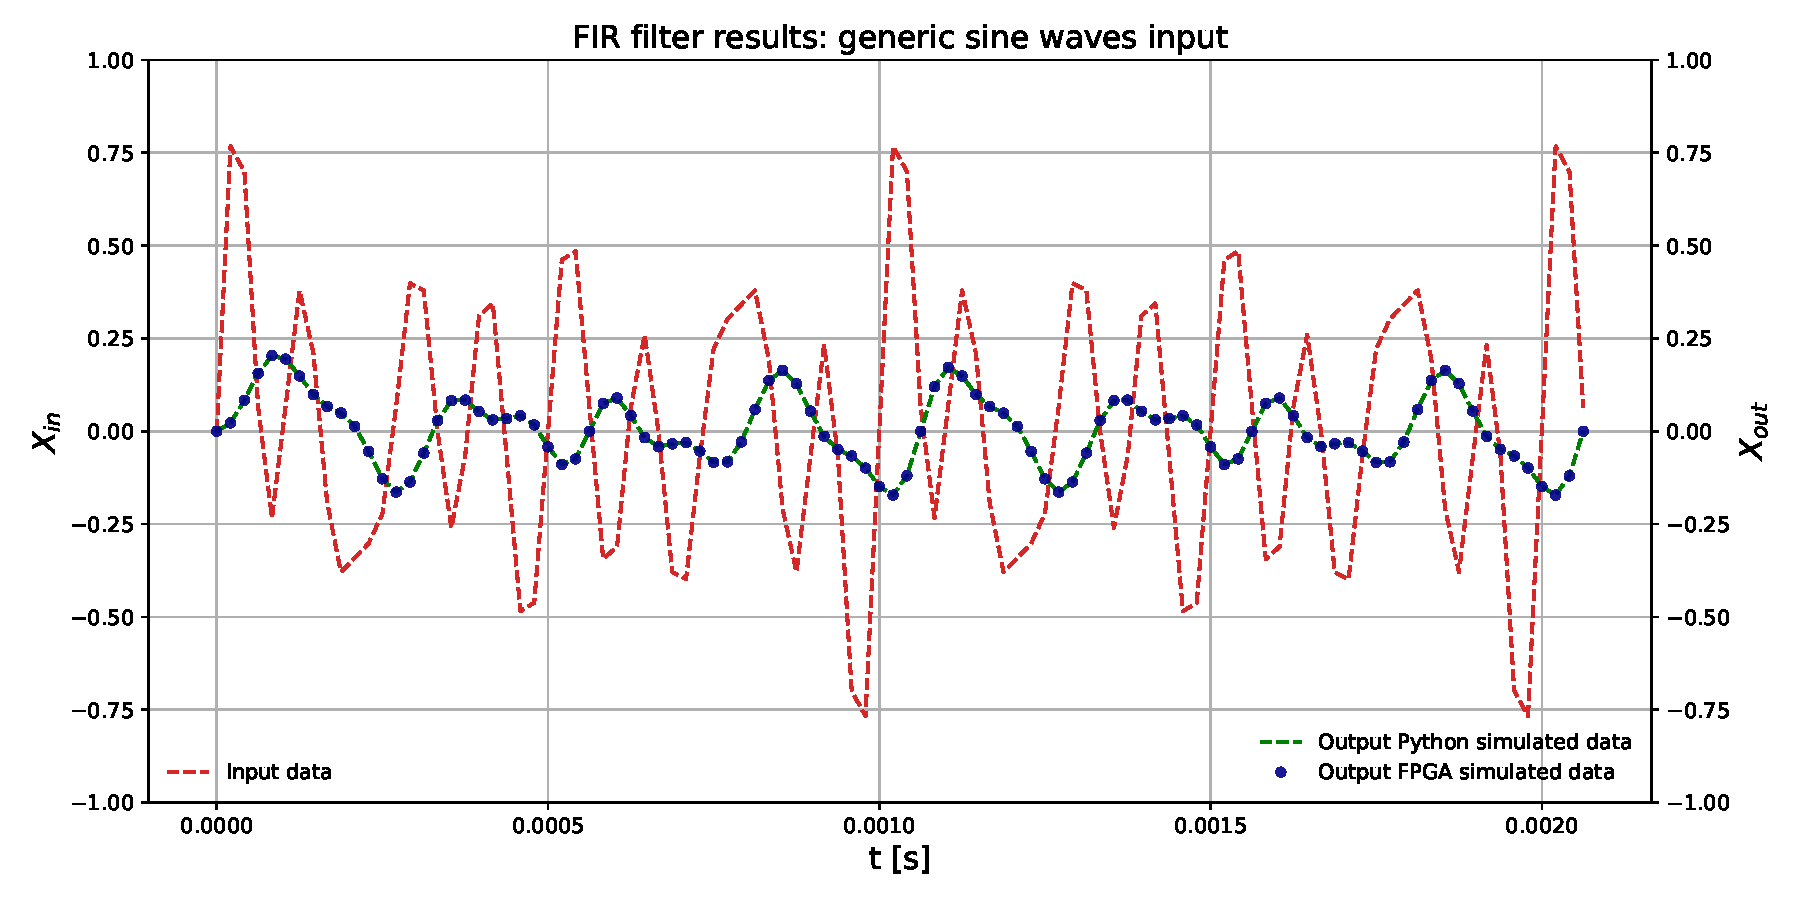
\includegraphics[width=1.0\textwidth]{images/FIR_out.pdf}
    \caption{FIR filter response with a generic sine waves.}
    \label{fig:FIR_response}
\end{figure}

\begin{figure}[!h]
    \centering
    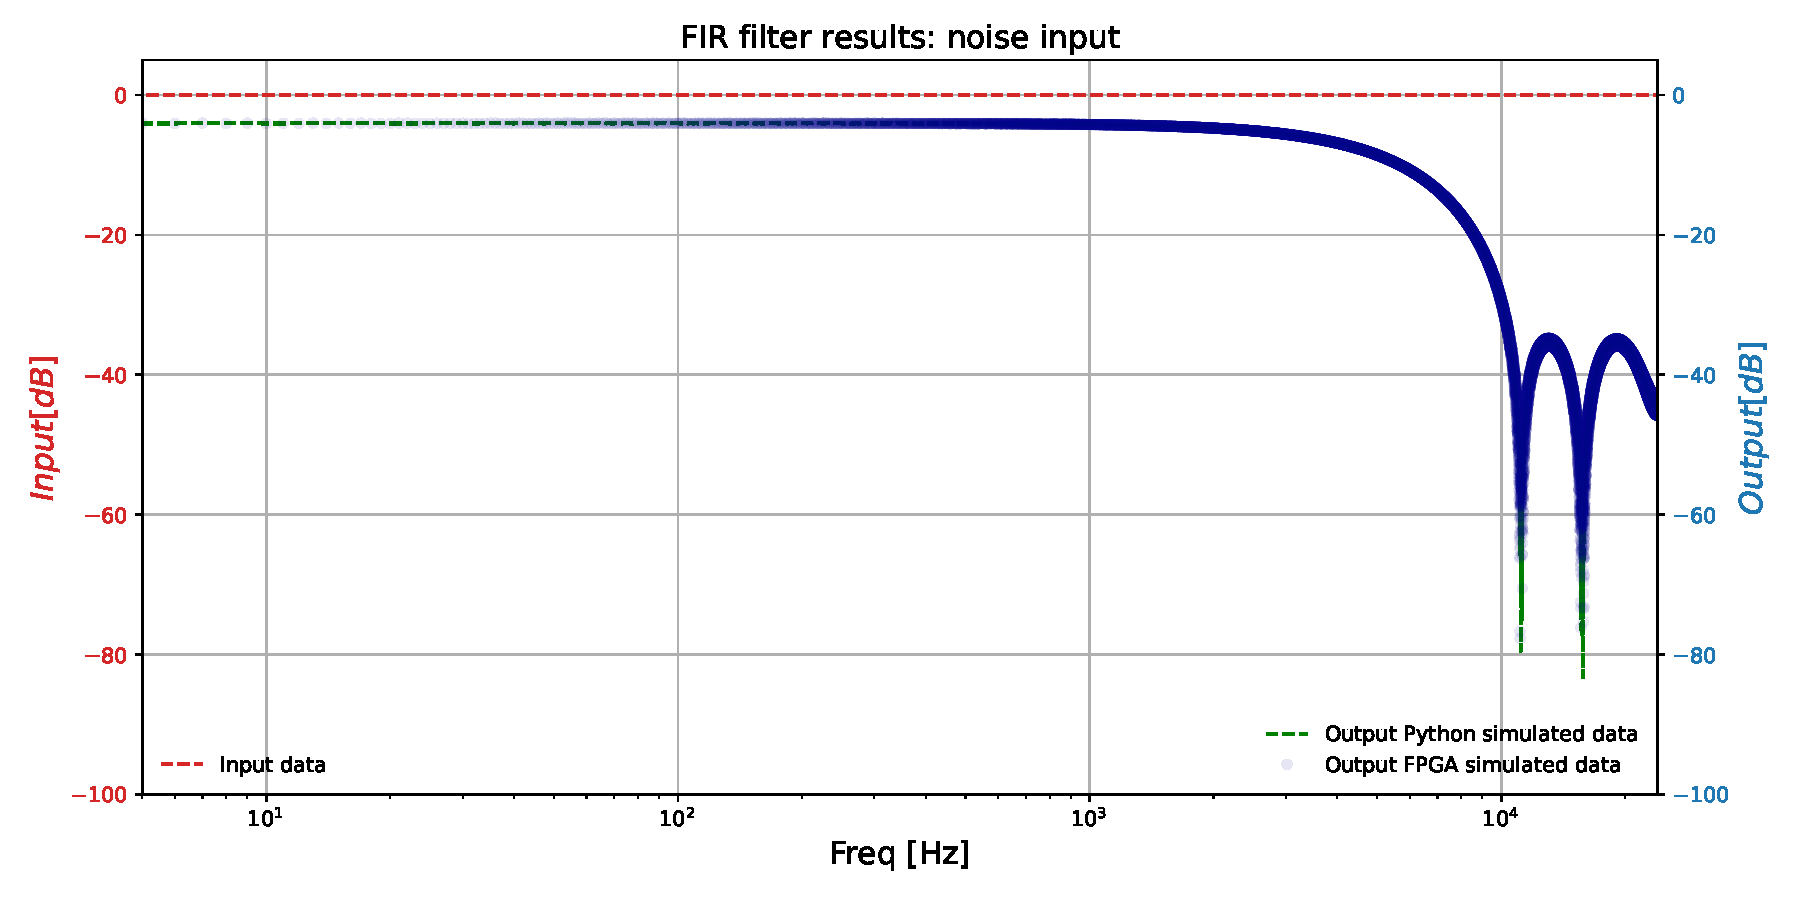
\includegraphics[width=1.0\textwidth]{images/fft_plot_log.pdf}
    \caption{Frequency analysis of the FIR filter with the given configuration.}
    \label{fig:FIR_freq_analysis}
\end{figure}

\subsection{Real-world validation}

The filter has been finally tested with real audio data samples. In particular, 31 different frequencies were sent to the FPGA and the output RMS values have been measured with an oscilloscope.  

The output has been then rescaled computing the logarithm, in order to match the simulation data. The values in mV and dB are given in the table below.

\begin{figure}[!h]
    \centering
    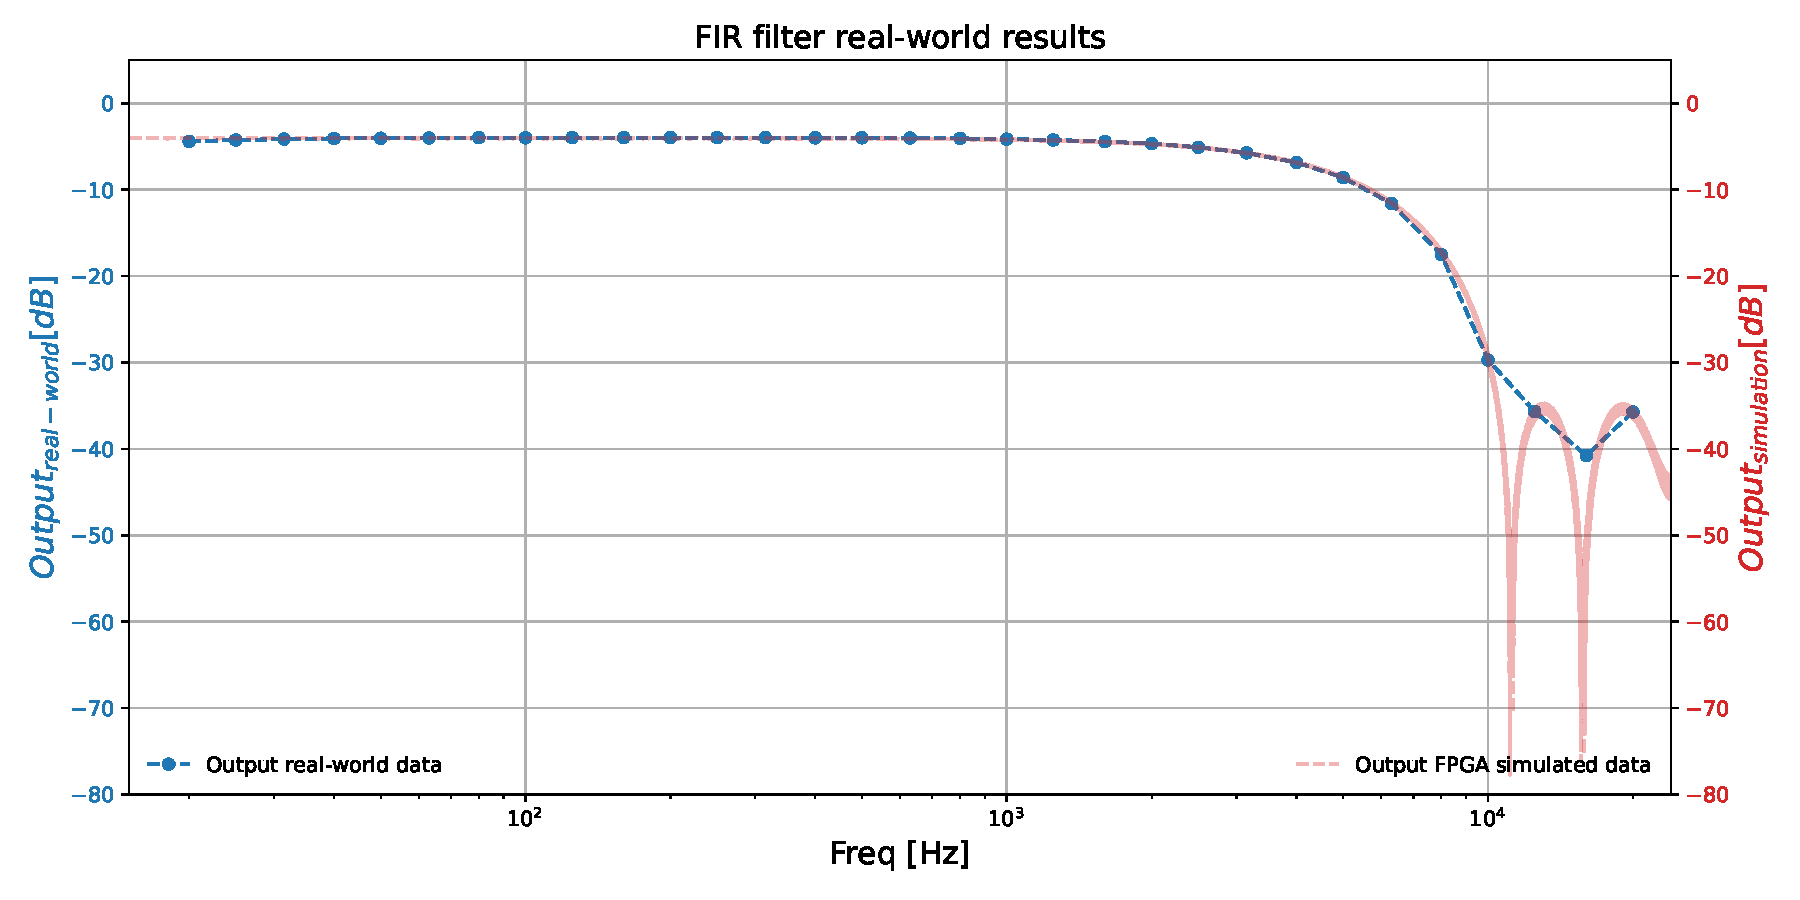
\includegraphics[width=1.0\textwidth]{images/real_wolrd_plot_log.pdf}
    \caption{FIR filter response with different input sine wave frequencies}
    \label{fig:FIR_real-wolrd}
\end{figure}

From plot \ref{fig:FIR_real-wolrd}, it is clear that the filter responds as expected, but at higher frequencies the oscilloscope's resolution hides the real filter's behaviour.

% table here


\section{Conclusion}
In this assignment we presented two different architectures of a FIR filter, implemented in FPGA hardware. We also exploited I$^2$S protocol and modules provided by Digilent to exchange and sample the audio stream.

\begin{thebibliography}{99}
    
        \bibitem{Digilent} 
        Digilent website, 
        \url{https://digilent.com/reference/pmod/pmodi2s2/start?redirect=1}
        
        \bibitem{Fir_github}
        Github repository, 
        \url{https://github.com/Gabriele-bot/MAPD_LAB/tree/main/FIR_project}
        
    \end{thebibliography}

\end{document}
